\documentclass[letterpaper,12pt]{article}

\usepackage{ge05}
\usepackage{comment}
\usepackage{booktabs}
\usepackage[dvipdfm]{hyperref}
\urlstyle{rm}   % change fonts for url's (from Chad Jones)
\hypersetup{
    colorlinks=true,        % kills boxes
    allcolors=blue,
    pdfsubject={NYU Stern course GB 2303, Global Economy},
    pdfauthor={Dave Backus @ NYU},
    pdfstartview={FitH},
    pdfpagemode={UseNone},
%    pdfnewwindow=true,      % links in new window
%    linkcolor=blue,         % color of internal links
%    citecolor=blue,         % color of links to bibliography
%    filecolor=blue,         % color of file links
%    urlcolor=blue           % color of external links
% see:  http://www.tug.org/applications/hyperref/manual.html
}

\newcommand{\GDP}{\mbox{\em GDP\/}}
\newcommand{\NDP}{\mbox{\em NDP\/}}
\newcommand{\GNP}{\mbox{\em GNP\/}}
\newcommand{\NX}{\mbox{\em NX\/}}
\newcommand{\NY}{\mbox{\em NY\/}}
\newcommand{\CA}{\mbox{\em CA\/}}
\newcommand{\NFA}{\mbox{\em NFA\/}}
\newcommand{\Def}{\mbox{\em Def\/}}
\newcommand{\CPI}{\mbox{\em CPI\/}}

\def\ClassName{The Global Economy}
\def\Category{Class Notes}
\def\HeadName{Solow's Growth Model}

\begin{document}
\parskip = 0.7\bigskipamount 
\thispagestyle{empty}%
\Head

\centerline{\large \bf Solow's Model of Economic Growth}%
\centerline{Revised:  \today}

\bigskip
We see large differences in saving and investment rates across
countries, with (for example) the US investing 20\% of GDP,
China 30\%, and India 12\% in recent years
(ratios of real investment to real GDP from the Penn World Tables).
How important are these differences to the income and growth rates of countries?
The answer:  not very important.
Why?  Because diminishing returns to capital means
(in practice) that additional capital generates smaller and smaller
additions to output.
That's somewhat disappointing, but is nevertheless useful because it tells
us to look elsewhere if we want to account for the enormous differences
we see across countries.  
The insight comes from Robert Solow,
the 1987 recipient of the Nobel Prize in economics.


\subsubsection*{The model}
%
Solow's model has four relatively simple components.
The first is our friend the production function:
\begin{equation}
    Y_t \;=\; A_t F(K_t,L_t) \;=\; A_t K_t^{\alpha} L_t^{1-\alpha}.
        \label{eq:pf}
\end{equation}
Changes in output therefore come from changes in
(total factor) productivity, capital, and/or labor.
Recall that one of the properties of this production function
is diminishing returns to capital:
each additional unit of capital leads to a smaller addition to output.
This is the critical ingredient in what follows.
The second component is a link between investment and saving.
You'll recall that the flow identity,
$
    S_t \;=\; I_t + (G_t-T_t) + \NX_t ,
$
linked household or personal saving to 
investment, the government deficit, and net exports.
(In an earlier note we called $S$ personal saving
and labelled it $S_p$, but we'll skip the subscript here.)
Solow ruled out the last two (we can put them back in later if we like),
giving us
\[
    S_t \;=\; I_t.
\]
Lurking behind the scenes here is the expenditure identity,
$ Y_t = C_t + I_t$ in this case.
The third component is a description of saving behavior:
people save a constant fraction $s$ of their income,
\[
    S_t \;=\; s Y_t,
\]
where the saving rate $s$ is a (constant) number between zero and one.
This is a little simplistic ---
you might expect saving to depend on
the rate of return and/or expectations of future income ---
but simplicity has a lot to be said for it.
For our purposes, $s$ is really the investment rate (the ratio of
investment to GDP), but since saving and investment are the same
here, we can call it the saving rate.
Finally, the capital stock depreciates at a constant rate $\delta$,
so that
\[
    K_{t+1} \;=\; (1-\delta) K_t + I_t ,
\]
where the depreciation rate $\delta$ is a number between zero and one.


The model consists of these four equations.
This seems kind of simple for a Nobel Prize, but they really are good equations.
Now let's see where they lead.


\subsubsection*{Capital dynamics}
%
Let's think about how the model behaves if the labor input $L$
and productivity $A$ are constant.
Analysis of the model in this case consists of describing
how the capital stock evolves through time.
Other variables follow from their relations to the capital stock:
we can find output from the production function,
saving (= investment) from output,
and consumption from the expenditure identity ($ Y_t = C_t + I_t$).
All of this is easily done in a spreadsheet.

The key step is to describe how the capital stock changes from one period to the next.
With a little work, we see that the capital stock behaves like this:
\begin{eqnarray}
    K_{t+1} &=& (1-\delta) K_t + I_t \nonumber \\
            &=& (1-\delta) K_t + S_t \nonumber  \\
            &=& (1-\delta) K_t + s Y_t \nonumber \\
            &=& (1-\delta) K_t + s A K_t^\alpha L^{1-\alpha} .
            \label{eq:k-lom}
\end{eqnarray}
Note that each step follows from one of the components of the model.
[Suggestion:  label them yourself
to make sure you follow the logic.]
%For practice, you
If we have values for the parameters $(A,\alpha,s,\delta)$,
we can program this up and see how $K$ moves through time.


{\it Example\/}. A numerical example --- a ``simulation'' ---
will show you how this works.
Let $L = 100$, $ A = 1$, $s = 0.2$, $\delta = 0.1$, and $\alpha =
1/3$. (We'll use the same parameters throughout.) If the initial
capital stock is 250, we can compute future values of the capital
stock by applying equation (\ref{eq:k-lom}) repeatedly.
We then compute output from the capital
stock using the production function, equation (\ref{eq:pf}). 

The results for this case are
summarized in Table~\ref{tab:example}.
%
\tabcolsep = 0.1in
\begin{table}[h]
\begin{center}
\begin{tabular}{ccc}
\toprule
Date $t$  &  Capital Stock $K$ &  Output $Y$ \\
\midrule 
    0 & 250.0 & 135.7 \\
    1 & 252.1 & 136.1 \\
    2 & 254.2 & 136.5 \\
    3 & 256.0 & 136.8 \\
    4 & 257.8 & 137.1 \\
    5 & 259.4 & 137.4 \\
    6 & 261.0 & 137.7 \\
    7 & 262.4 & 137.9 \\
    8 & 263.8 & 138.2 \\
    9 & 265.0 & 138.4 \\
   10\phantom{0} & 266.2 & 138.6 \\
%   11 & 267.2864 & 138.7796 \\
%   12 & 268.3136 & 138.9572 \\
%   13 & 269.2737 & 139.1227 \\
%   14 & 270.1709 & 139.2770 \\
%   15 & 271.0092 & 139.4209 \\
%   16 & 271.7925 & 139.5551 \\
%   17 & 272.5242 & 139.6803 \\
%   18 & 273.2079 & 139.7970 \\
%   19 & 273.8465 & 139.9058 \\
%   20 & 274.4430 & 140.0073 \\
\bottomrule 
\end{tabular}
\end{center}
\caption{Simulation of the Solow model.}
\label{tab:example}
\end{table}
%
[Suggestion:  try to reproduce a couple periods of the table to
make sure you understand how it works.
If you get stuck, read the last two pages again.
The trick is to set up formulas that tie each period to the previous one.]
You can see in the table
that capital and output both increase over time.
Will they increase forever?
The answer is no, but it takes a little work to
show. (Alternatively, you could extend the simulation and see what
happens.)
This is an important conclusion, because it tells us saving
and capital formation can't be the reason
(in this model, anyway)
that some countries grow faster than others --- indefinitely.
More on this soon.


The dynamics of the capital stock reflect a balance of two factors:
(i)~saving tends to increase the capital stock by financing new investment
and (ii)~depreciation tends to reduce it.
We see why if we subtract $K_t$ from both sides of equation (\ref{eq:k-lom}):  
\begin{eqnarray}
    \Delta K_{t+1} &=& K_{t+1} - K_t
            \;=\;  s A K_t^\alpha L^{1-\alpha} - \delta K_t .
            \label{eq:dK}
\end{eqnarray}
You can see that the change is zero (the capital stock doesn't change)
when $ \Delta K_{t+1} = 0$ or
\begin{eqnarray}
    K_{ss} &=& \left( {s A}/{\delta} \right)^{1/(1-\alpha)} L ,
        \label{eq:Kss}
\end{eqnarray}
where $K_{ss}$ is the ``steady state'' capital stock.
This is a little complicated, but remember, it's just a formula.
In our example, $K_{ss} = 282.8$, so we have a ways to go before the model reaches its steady state.

\begin{comment}
Since $A$ and $L$ are constant, when capital is at a steady state,
output is, too.
Its value is
\begin{eqnarray}
    Y_{ss} &=&  A K_{ss}^\alpha L^{1-\alpha} \nonumber \\
           &=&  A^{1/(1-\alpha)}
                \left( {s}/{\delta} \right)^{\alpha/(1-\alpha)} L .
        \label{eq:ss-y}
\end{eqnarray}
(The second line comes from substituting for $K_{ss}$,
but it takes a little work to get there.)
That gives us the steady state capital-output ratio,
\begin{eqnarray*}
    K_{ss}/Y_{ss} &=&  \left( {s}/{\delta} \right) .
\end{eqnarray*}
(This also takes some work,
but at least it's mercifully simple when we get there.)
This is a number we can do something with.  Typically countries have
relatively stable capital-output ratios ---
numbers like 2 or 3 ---
so we can compare them to the evidence.
We can ask, for example, how much a higher saving rate increases
the capital intensity of a country,
using the capital-output ratio as a measure of capital intensity.
We'll do that in the section after next.
\end{comment}

\begin{figure}[h]
    \centering
    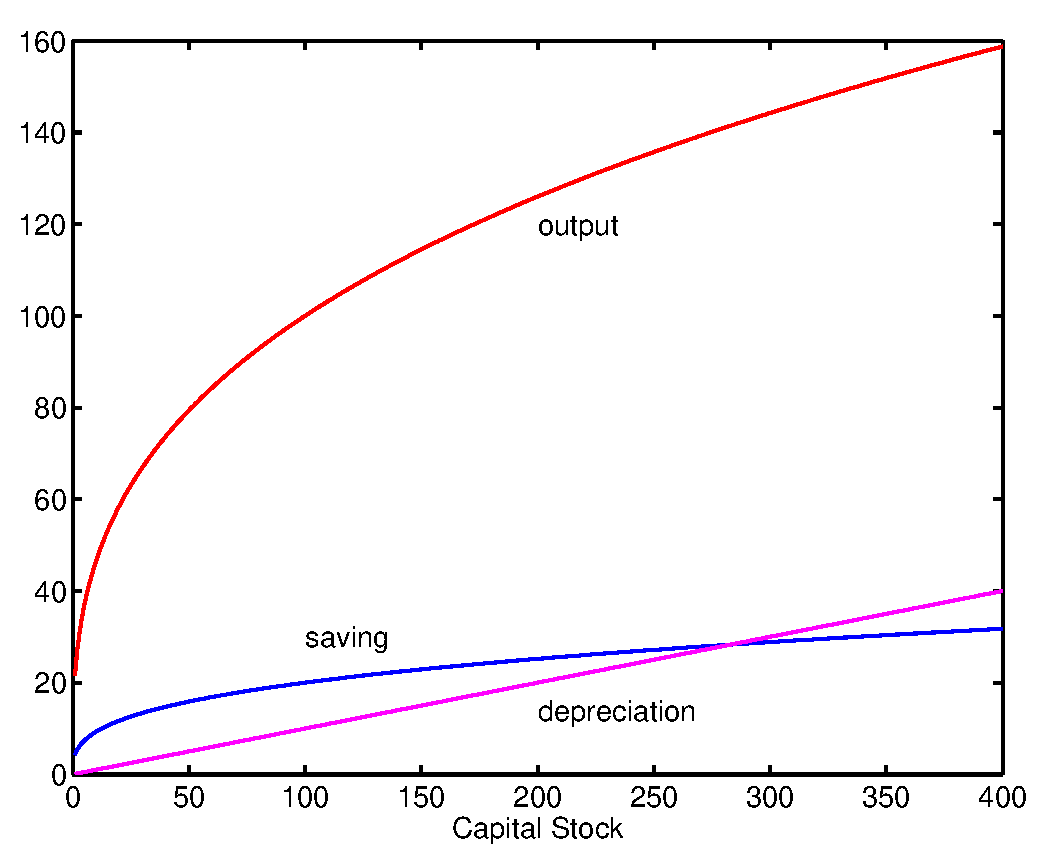
\includegraphics[scale=.6]{notes_solow1.eps}\\
    \caption{The Solow model.}
    \label{fig:solow1}
\end{figure}

Let's return to dynamics.
What happens if we are above or below $K_{ss}$?
You can get a sense of the dynamics from Figure~\ref{fig:solow1}.
The top line is output,
which is related to the capital stock through the production function.
The next line is saving, a constant fraction of output
and the first expression on the right side of equation (\ref{eq:dK}):  
$s A K_t^\alpha L^{1-\alpha} $.
The third line is depreciation, a constant fraction $\delta$
of the capital stock and the second object on the right side of equation (\ref{eq:dK}):  $\delta K_t $.
Diminishing returns to capital gives the saving line its curvature.
It leads to higher saving than depreciation at low
values of the capital stock, so the capital stock is increasing.
Similarly, saving is lower than depreciation at high values of the capital stock,
so the capital stock falls.
The crossing point is $K_{ss}$, where saving is just enough to
make up for depreciation, leaving the capital stock unchanged.


\subsubsection*{Impact of saving and investment on income}

So what have we seen?
We've seen that if productivity $A$ and labor input $L$ are constant, 
the saving rate has no impact on the long-term growth of the economy.
At least in this model, the capital stock (and therefore output) will eventually 
converge to its steady state value and the economy will not grow.  
Differences in saving rates are therefore not 
an explanation of the differences we see in growth rates across countries.  
That's not to say saving is irrelevant, but it
can't be the primary factor in country performance.  

So if saving has no impact on long-term growth, what does it do?  
It affects the level of income.  
Countries with higher saving rates have higher steady state capital stocks 
and therefore higher steady state income.  
We can see that in Figure \ref{fig:solow1a}.
The solid lines at the bottom are the saving and depreciation
lines from the previous figure.  
They cross at the steady state capital stock.  
The top line (the dashed one) shows what happens to saving if we increase 
the saving rate from 0.2 to 0.25.  
Saving is higher at every value of the capital stock.  
As a result, the steady state capital stock (where the dashed line crosses
depreciation) is higher.  
And since capital is higher, output will be higher, too.  

We can see the same thing in the mathematics.  
Equation (\ref{eq:Kss}) shows how the steady state capital stock varies 
with the saving rate.  
Evidently higher saving leads to a larger stock of capital.  
If we plugged in numbers, we'd see that 
steady state output rises by 11\%.
That's not irrelevant, but it's a relatively modest increase
for a significant increase in saving.

\begin{figure}[h]
    \centering
    \includegraphics[scale=.6]{notes_solow1a.eps}\\
    \caption{The impact of higher saving in the Solow model.}
    \label{fig:solow1a}
\end{figure}


\subsubsection*{Growth}

If saving doesn't generate growth, what does?
We add growth in the labor force and
(critically) growth in total factor productivity
with two goals in mind.
The first goal is to account for the growth rate of output,
showing how it depends on the growth rates of our two inputs.
The second is to show that the economy approaches
what we call a balanced growth path in which
output and capital grow at the same rate.
As before, the capital-output ratio approaches a constant,
whose features we can easily summarize.
We do this with a striking example in mind:
we know that China invests an astounding 40\% of its GDP.
Is this too much?
A hint of the answer is that capital intensity
(measured by the capital-output ratio)
depends not only on the investment rate (which tells us how
much new capital is added) but on the growth rate
(how fast the denominator is changing).
A fast-growing economy needs a high investment rate
simply to maintain a given capital-output ratio.


We start with some ugly algebra (sorry), 
then return to the issue of China.  
The new inputs into our analysis are growth in the labor force
and productivity.
Let us say, to be concrete,
that labor and productivity grow
at constant rates:
\begin{eqnarray*}
    L_{t+1} &=&  (1+n) L_t \\
    A_{t+1} &=&  (1+a) A_t .
\end{eqnarray*}
How fast do output and capital grow?
Let's guess that output and capital grow at the same rate $g$,
to be determined.
(Why?  Because we're good guessers.)
From the production function, we then know
\begin{eqnarray*}
    (1+g)       &=& Y_{t+1}/Y_t  \\
                &=&  (A_{t+1}/A_t) (K_{t+1}/K_t)^\alpha
                        (L_{t+1}/L_t)^{1-\alpha} \\
                &=& (1+a) (1+g)^{\alpha} (1+n)^{1-\alpha} .                        \end{eqnarray*}
The growth rate is therefore
\begin{eqnarray*}
    (1+g)       &=& (1+a)^{1/(1-\alpha)} (1+n) .                        \end{eqnarray*}
Just a formula, but it says that output growth is tied
to the growth rates of productivity and labor.
Note, once again, that the saving rate does not affect this growth rate.
Similarly, the growth rate in output per worker is
\begin{eqnarray*}
    (1+g)/(1+n)     &=& (1+a)^{1/(1-\alpha)} ,                        \end{eqnarray*}
which depends only on productivity growth.
If $a$ is positive,
the growth rate of output per worker is
higher than the growth rate of productivity,
because the exponent $ 1/(1-\alpha)$ is greater than one.
In words:  the direct impact of productivity on output
is magnified by the growth in the stock of capital;
see the production function (\ref{eq:pf}).
This ties in with a remark we made earlier note:
that capital accumulation
tends to reinforce the impact of productivity growth.
%Countries with high productivity also have a lot of capital.


What about capital:
Do countries with high saving rates have more
capital, relative to the size of their economies?
The answer is yes, but it's also true that 
fast-growing countries need to invest a lot simply to maintain
a constant ratio of capital to output.
China has a large investment rate, but it needs it to maintain a
capital-output ratio comparable to the US.
If you buy that, you can safely skip the rest of the section.

Consider, again, a ``steady state'' in which capital and output grow
at the same rate $g$.
Then equation (\ref{eq:k-lom}) becomes
\begin{eqnarray*}
    K_{t+1}  &=& (1-\delta) K_t + s Y_t  \\
    (1+g) K_t/Y_t &=& (1-\delta) K_t/Y_t + s .
\end{eqnarray*}
Solving for $K/Y$ gives us the steady state capital-output ratio:
\begin{eqnarray}
    (K/Y)_{ss} &=& \left( \frac{s}{\delta+g} \right) .
    \label{eq:ky-ss-g}
\end{eqnarray}
You may note that this line of argument doesn't actually
require the Solow model:
all we need is the equation connecting capital today to capital tomorrow.
If we divide equation (\ref{eq:k-lom})
by $Y_t$ and substitute $ Y_{t} =  Y_{t+1}/(1+g)$, we get
\begin{eqnarray*}
    (1+g) K_{t+1}/Y_{t+1}  &=& (1-\delta) K_t/Y_t + s .
\end{eqnarray*}
The steady state capital-output ratio
(the ratio that makes $K_{t+1}/Y_{t+1}$ and $K_{t}/Y_{t}$ equal)
is exactly what we just derived.


To return to our goal of understanding the sources of capital intensity,
note the impact of growth on the steady state capital-output ratio.
For a giving saving/investment rate $s$, countries with higher growth
will have relatively less capital per unit of output.
Why?  Because output is growing quickly,
you need to invest a lot to keep capital in line with output.


{\it Example.}
Here are some numbers based loosely on the US:
$ n = 0.005 $ (0.5\%), $ a = 0.01 $ (1\%), $s=0.15$,
and $\delta = 0.06$.
What is the growth rate of the output?
The steady state capital-output ratio?
The growth rate satisfies
\[
    1+g \;=\; (1+a)^{1/(1-\alpha)} (1+n) \;=\; 1.015 \times 1.005
        \;=\; 1.0201.
\]
Here we've used $\alpha = 1/3$, as usual.
Using the same parameters as our earlier examples, the steady state
capital-output ratio is
\[
    1.872 \;=\; \frac{0.15}{0.06 + 0.020} .
\]
Now consider numbers based on China.
We keep $ n = 0.005 $ and $\delta = 0.06$,
but change the others to $ a = 0.06 $ and $s = 0.30 $.
The growth rate is now $g = 0.0968$ and the capital-output ratio
falls to 1.013.
Note the modest increase, despite the large increase in the
saving/investment rate.
Is China saving too much?
Maybe not:  their capital-output ratio (by this calculation)
is not much different from that in the US.
They need to invest a lot simply to keep up with the growth
of their economy.


%\subsubsection*{Discussion}


%[??] Solow's work focussed attention on saving and investment.
%If high per capita income required high saving, then maybe we should save more.
%And if it required investment, poor countries should think about
%financing investment through foreign borrowing as well as domestic saving.
%Our sense is that neither of these conclusions are supported by the evidence.
%High saving rates do finance greater investment,
%but they come at the cost of lower consumption rates.
%And poor countries, as we'll see, are poor primarily because they
%have low productivity, not because they lack capital.


\subsubsection*{Executive summary}

\begin{enumerate}
\item Solow's model bases growth on saving and investment.

\item Saving has a modest impact on steady state capital and output, 
and none on their growth rate.

\item
Fast-growing countries must save and invest more than slower-growing countries
to have maintain the same capital-output ratio.
\end{enumerate}

%\end{document}

\subsubsection*{Review questions}

\begin{enumerate}

\item For the numerical example in the text:
\begin{enumerate}
\item Suppose the economy starts with the steady state capital stock.
What are the steady state levels of output, investment, and consumption?
\item If 25\% of the capital stock is destroyed in a war,
how much does output fall?
How long does it take the economy to reverse half the fall in output?
\end{enumerate}

Answer.
\begin{enumerate}
\item The steady state capital stock is (as we've seen) $K_{ss} = 282.8$.
Using this value, the production function tells us that output is 141.4.
Investment equals the depreciation of the capital stock, 28.3.
We can find consumption two ways.
The first is through the expenditure identity:  $Y = C + I$.
We know $Y$ and $I$, so $C$ is 113.1.
The second is through the flow identity.
Saving is fraction $s$ of output, so consumption is fraction $1-s$,
$ 0.8 \times 141.4 = 113.1 $.

\item This requires a simulation.
Let the capital stock fall to 212.1, 75\% of its steady state value.
Then output falls to 128.5, 90.9\% of its steady state value.
We recover half the fall if output rises to 135.0.
If we simulate the model, we see that it reaches 135.1 in 10 periods
(years).
\end{enumerate}


\item We've ignored government so far.  Suppose, instead,
that the government purchases goods and services
equal to a constant fraction of GDP
(say, $ G = g Y$ for some fraction $g$)
 and collects taxes equal to the same fraction of output.
Individuals have after-tax income of $ (1-g) Y$ and save a
fraction $s$ of it.
With these changes, how would the analysis of the basic Solow model change?

Answer.  The critical ingredient here is the fraction of output allocated
to investment.
Investment here is $ I = S = s (1-g) Y $.
Effectively, $g$ reduces the saving rate from $s$ to $s(1-g)$
and takes resources away from investment.
If the government invests, we'd have to include that,
but we'd also have to decide how useful the investment was
(does it count the same as other investment?).

\item (optional) Consider the model with population growth, and suppose
$\delta = 0.1$, $s = 0.2$, $A = 1$, and $n = 0.01$. How much does
steady state output per worker fall if $n$ rises to 0.02? \\
Warning:  This is moderately difficult.
You need to work out the steady state on your own,
not apply a formula in the notes.

Answer.  With $n=0.01$, steady state output per worker is 1.348.
When $n=0.02$, it falls to 1.291, a drop of about 4\%.

\end{enumerate}

%\end{document}

\subsubsection*{If you're looking for more}

The Solow model is covered in most macroeconomics textbooks.
%
It's sometimes used as a forecasting tool.
It doesn't make forecasting any less hazardous than usual, 
but it tells us what the critical inputs are.
The critical one, of course, is productivity growth.
Goldman Sachs did this a few years back to estimate the importance of
the BRICs (Brazil, Russia, India, and China) in the world economy.  
See their 
\href{http://www2.goldmansachs.com/our-thinking/brics/brics-at-8/index.html}
{BRICs page}.


\vfill \centerline{\it \copyright \ \number\year \  NYU Stern
School of Business}

\end{document}
